\documentclass[11pt]{beamer}
\usetheme{default} 

\setbeamertemplate{navigation symbols}{} %gets rid of navigation symbols
\setbeamertemplate{footline}{} %gets rid of bottom navigation bars
\setbeamertemplate{footline}[page number]{} %use this for page numbers

\setbeamertemplate{footline}{%
  \raisebox{5pt}{\makebox[\paperwidth]{\hfill\makebox[10pt]{\scriptsize\insertframenumber~~}}}}

\setbeamertemplate{itemize items}[circle] %round bullet points
\setlength\parskip{10pt} % white space between paragraphs

\usepackage{wrapfig}
\usepackage{subfig}
\usepackage{setspace}
\usepackage{enumerate}
\usepackage{graphicx}
\usepackage{amsmath}
\usepackage{amsfonts}
\usepackage{amssymb}
\usepackage{amsthm}
\usepackage[UKenglish]{isodate}
\usepackage{tikz}
\usepackage{pgfplots}
\usepackage{natbib}
\def\checkmark{\tikz\fill[scale=0.4](0,.35) -- (.25,0) -- (1,.7) -- (.25,.15) -- cycle;} 

% allow drawing arrows
\usetikzlibrary{arrows}
\usetikzlibrary{shapes.arrows}
\tikzstyle{arrow}=[draw, -latex] 

\tikzset{
    myarrow/.style={
        draw,
        single arrow,
        minimum height=5ex,
        single arrow head extend=1ex
    }
}

% skips
\setlength{\abovecaptionskip}{15pt plus 3pt minus 2pt}
\setlength{\belowcaptionskip}{5pt plus 3pt minus 2pt}
% bracketing shortcuts
\newcommand{\paren}[1]{\left(#1\right)}
\newcommand{\sqbracket}[1]{\left[#1\right]}
\newcommand{\cbracket}[1]{\left\{#1\right\}}
\newcommand{\abs}[1]{\left\lvert#1\right\rvert}
\newcommand{\norm}[1]{\left\lVert#1\right\rVert}
% set up the argmin operator, argmax
\DeclareMathOperator*{\argmin}{arg\,min}
\DeclareMathOperator*{\argmax}{arg\,max}

\newcommand{\myframe}[1]{\begin{frame} \frametitle{#1}}
% New itemize environment, with spaces
\newenvironment{spaceitemize}
{ \begin{itemize}
    \setlength{\itemsep}{10pt}
    \setlength{\parskip}{0pt}
    \setlength{\parsep}{0pt}     }
{ \end{itemize}                  } 

% the preamble
\title{Day 2, Session 1: Logs/Exponentiation}
\author{Jessica Williams-Nguyen and Brian D. Williamson}
\institute{EPI/BIOST Bootcamp 2018}
\date{24 September 2018}

% Start the document
\begin{document}
% The title page
\begin{frame}
\titlepage
\end{frame}

\section{Introduction}
\myframe{Motivation}
Generally, our goal in a statistical analysis is to \textcolor{blue}{assess an association} between two variables (e.g., smoking and lung cancer). We can do this by investigating whether a \textcolor{green}{summary measure} (e.g., mean, median) of our outcome (e.g., lung cancer) is \textcolor{cyan}{unequal between two groups} differing in our predictor of interest (e.g., smoking). \pause

There are two simple ways to tell if two numbers are unequal: 
\begin{itemize}
\item their difference is not equal to 0, or \pause
\item[]
\item their ratio is not equal to 1.
\end{itemize}

We choose between these based on a variety of criteria, which fall into two general categories: (1) adequately address the scientific question, and (2) gain desirable statistical properties.
\end{frame}

\myframe{Motivation}
Differences:
\vspace{-0.5cm}
\begin{spaceitemize}
\item are \textcolor{blue}{generally easier to understand}, and \pause
\item are better for describing the \textcolor{cyan}{scientific importance} of many comparisons
\begin{itemize}
\item You probably always want \$1,000,000 more than me, even if I have \$10,000,000 (a ratio of 1.1)
\end{itemize}
\end{spaceitemize} \pause
Ratios work well when working with \textcolor{green}{small numbers} (disclaimer: these numbers are probably only correct to the order of magnitude, but get the point across); for example: \pause
{\fontsize{10pt}{7.2}\selectfont
\begin{itemize}
\item In the US, 60--64 year old current or former smokers have a probability of 0.00296 of being diagnosed with lung cancer during the next year \pause
\item In the US, 60--64 year old never smokers have a probability of 0.000148 of being diagnosed with lung cancer during the next year \pause
\item Difference in incidence rates: 0.002812; ratio of incidence rates: 20!
\end{itemize}
}
\end{frame}

\myframe{Motivation}
Sometimes, the \textcolor{cyan}{scientific mechanism} dictates that \textcolor{blue}{ratios are more generalizeable}: \pause
{\fontsize{10pt}{7.2}\selectfont
\begin{itemize}
\item Interventions or risk factors that affect a rate over time (e.g., HIV incidence)
\item[] \pause
\item Biochemical processes (e.g., rates of absorption, where the rate is proportional to drug concentration) 
\end{itemize}
}
\pause
When ratios are scientifically preferred, we can use the \textcolor{red}{logarithm of the ratio} to get back to \textcolor{purple}{comparing differences} (more on this later).
\end{frame}

\myframe{Common variables}
Some variables are almost always log transformed: \pause
\begin{itemize}
\item Acidity/alkalinity of an aqueous solution: measured as hydrogen ion concentration, but pH usually reported [$-\log_{10}(\text{H ion conc.})$]
\item[] \pause
\item Concentrations of antibodies or mRNA: these differ by orders of magnitude across people, and within people over time
\end{itemize}
\pause
Properties of exponentiation and logarithms come in handy throughout statistics and data analysis; a solid understanding of the basics goes a long way.
\end{frame}

\myframe{Example: gender bias in salary {\small (from Scott Emerson, MD PhD)}}
We want to investigate the differences in salaries between male and female faculty members at the University of Washington for the years 1976--1995. The main question is \textcolor{red}{does discrimination in salaries exist in 1995}, based on a retrospective cohort study of 1,597 faculty members at the University of Washington. \pause

The average monthly salary for female faculty in 1995 was \$5,396.91; for male faculty, the average monthly salary in 1995 was \$6,731.64. \pause

There are a variety of potential confounding factors that we will consider: start year at UW, year of degree, field of study, highest degree, administrative duties, rank.
\end{frame}

\myframe{Example: gender bias in salary}
For our statistical analysis, we need to decide which is more meaningful: reporting \textcolor{green}{differences in mean salary}, or \textcolor{blue}{ratios of geometric mean salary}. \pause

Since salaries are expected to be somewhat comparable, perhaps with small differences, comparing salary on a multiplicative scale (i.e., ratios of geometric means) makes sense. \pause Also, we expect the difference between people who make \$1,000 and \$2,000 per month is more similar to the difference between \$10,000 and \$20,000 than the difference between \$2,000 and \$3,000. \pause This means we have to \textcolor{red}{log transform} the outcome! \pause

It also turns out that transforming the salary may give us more statistical precision, if the geometric mean is the correct comparison to make.
\end{frame}

\section{Exponentiation}
\myframe{Exponentiation}
Exponentiation corresponds to repeated multiplication, and is: \pause
\begin{itemize}
\item the second in the order of operations! (P\textcolor{blue}{{\textbf E}}MDAS)
\item[] \pause
\item composed of two numbers: a base, $b$, and an exponent, $n$ \pause
\begin{itemize}
\item represented as $b^n = \underbrace{b\times b \times \cdots \times b}_\text{$n$ times}$
\end{itemize}
\end{itemize} \pause

\textcolor{green}{Positive exponents multiply the base} $b$ a number of times given by $n$; \pause \textcolor{cyan}{negative exponents multiply the reciprocal of the base} $b$ a total of $n$ times. For example, $2^2 = 2\times 2$, and $2^{-2} = \left(\frac{1}{2}\right)^2 = \frac{1}{2}\times \frac{1}{2}$.
\end{frame}

\myframe{Properties of exponents}
\fontsize{9pt}{7.2}\selectfont
\begin{itemize}
\item If we multiply two numbers with the same base, we add their exponents \pause
\begin{itemize}
\item $10^3 \times 10^2 = 10^5$; $10^3 \times 10^{-2} = 10^1$
\end{itemize}
\item[] \pause
\item If we raise an exponentiated number to a power, we multiply the exponents; $(b^n)^m = b^{n\times m}$
\item[] \pause
\item The exponent can be a fraction (like $\frac{1}{2}$), which gives us the root of the base (if the base is positive) \pause
\begin{itemize}
\item $4^{1/2} = \sqrt{4} = 2$; $81^{1/4} = \sqrt[4]{81} = 3$
\end{itemize}
\item[] \pause
\item Multiplying different bases: first manipulate the exponent so the bases are equal, then add exponents \pause
\begin{itemize}
\item $2^3 \times 4^5 = 2^3 \times (2^2)^5 = 2^3 \times 2^{10} = 2^{13}$
\end{itemize}
\item[] \pause
\item For any $b, c \neq 0$: $b^0 = 1$, $(b \times c)^n = b^n \times c^n$
\end{itemize}
\end{frame}

\myframe{Exponential function}
\begin{itemize}
\item An important constant: $e$, approximately $2.718$
\item[] \pause
\item Useful as a base for powers
\item[] \pause
\item Define $\exp(x) = e^x$ as the \textcolor{blue}{exponential function}
\end{itemize}
\end{frame}

\myframe{Exercise: exponents and the exponential function}
\begin{enumerate}
\item What is the result of $x^2$ multiplied by $x^3$?
\item[]
\item $(x^{-2})^4 = $?
\item[]
\item $\exp(x - y) = $?
\end{enumerate}
\end{frame}

\myframe{Solutions: exponents and the exponential function}
\begin{enumerate}
\item $x^2 \times x^3 = x^5$, since we add the exponents when we multiply
\item[] \pause
\item $(x^{-2})^4 = x^{-2 \times 4} = x^{-8}$
\item[] \pause
\item $\exp(x - y) = e^{x - y} = e^x \times e^{-y} = e^x/e^y = \exp(x)/\exp(y)$
\end{enumerate}
\end{frame}

\section{Logs}
\myframe{Logarithms}
Logarithms (logs) \textcolor{blue}{transform multiplication into addition}. This leads to many of their mathematical properties. \pause

Before calculators, to multiply two large numbers (e.g., 1234 and 4747), you would: \pause
{\fontsize{10pt}{7.2}\selectfont
\begin{enumerate}
\item choose a common base (e.g., 10) \pause
\item convert each number into exponentiated form with this base (e.g., $10^{3.091315}$ and $10^{3.676419}$) using a table of logarithms (usually base 10) \pause
\item add the exponents (e.g., $3.091315 + 3.676419 = 6.767734$) \pause
\item convert back to un-exponentiated form (e.g., $10^{6.767734} = 5857798$) \pause
\end{enumerate}
}

The \textcolor{green}{logarithm} base 10 of a number is just the exponent of the number expressed as a power of 10; the logarithm base 10 of 100 is 2, because $10^2 = 100$.
\end{frame}

\myframe{Logs: definition}
More generally, we can define the \textcolor{blue}{logarithm base $k$ of a number $x$}, written $\log_k(x)$. If $\log_k(x) = y$, then $k^y = x$. \pause

Common convention in early math courses: 
\vspace{-0.4cm}
\begin{itemize}
\item ``log(x)'' is $\log_{10}(x)$, and \pause
\item ``ln(x)'' is the \emph{natural log}, $\log_e(x)$.
\end{itemize}  \pause

In many scientific applications, ``log(x)'' \textbf{is} $\log_e(x)$!
\vspace{-0.3cm}
\begin{itemize}
\item This is also true in most biostatistics courses and software
\end{itemize} \pause

Some basic properties of logarithms:
\vspace{-0.3cm} \pause
\begin{itemize}
\item undefined for $x \leq 0$
\item[] \pause
\item increasing: as $x$ increases, $\log_k(x)$ increases
\item[] \pause
\item $\log_k(k) = 1$
\end{itemize}
\end{frame}

\begin{frame}
\frametitle{Logs: definition}
\hspace*{-0.8cm}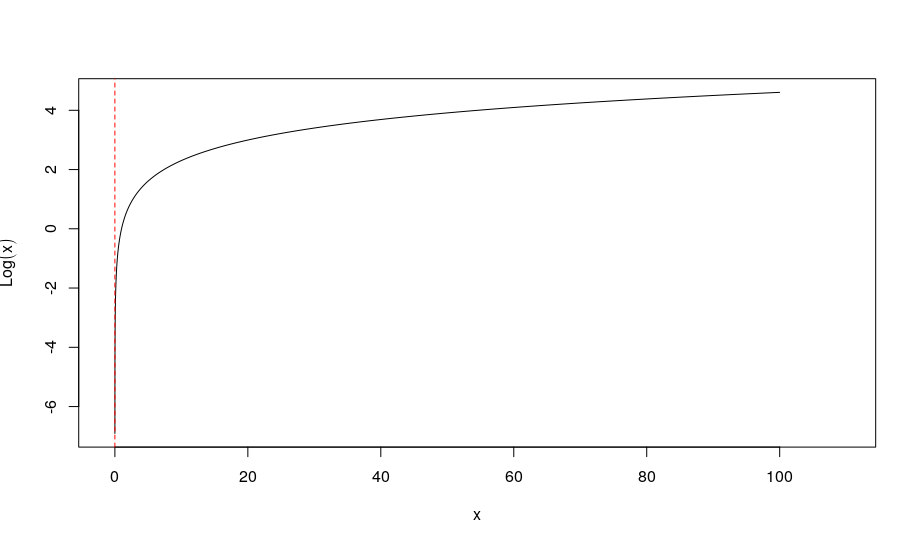
\includegraphics[width=1.2\textwidth]{figs/log.png}
\end{frame}

\myframe{Changing bases}
Using different bases for logarithms is similar to measuring length in different units (e.g., inches, centimeters). No matter what base you use, $\log(1) = 0$. \pause

This implies that we can convert between bases! This is often useful in science: if you transform a variable using log base $e$, you can change the base to 10 for a (potentially) more interpretable answer. \pause

We can find the base $k$ logarithm of any number using the most common bases ($e$ and 10): $\log_k(x) = \frac{\log_e(x)}{\log_e(k)} = \frac{\log_{10}(x)}{\log_{10}(k)}$. \pause
\end{frame}

\begin{frame}
\frametitle{Example: changing bases}
Suppose you have data on the FEV of children for various heights. You decide to log-transform (base $e$) height as you analyze the data. \pause

You could compare the average difference in FEV between two children who differ in age by 1 unit of log height. If this difference were 0.5 units, then there is, on average, a 0.5 unit difference in FEV for each $e$-fold increase in height. \pause

Equivalently, to find out the average difference in FEV for a 10\% increase in height, we find \vspace{-0.3cm}
\begin{align*}
\log_{1.1}(height) =& \ \frac{\log_e(height)}{\log_{e}(1.1)}
\end{align*}

and re-compute the average based on this new variable.

\end{frame}

\myframe{Logs: identities}
\begin{itemize}
\item Multiplication: $\log_b(xy) = \log_b(x) + \log_b(y)$
\item[] \pause
\item Division: for $y \neq 0$, $\log_b(x/y) = \log_b(x) - \log_b(y)$
\item[] \pause
\item Powers: $\log_b(x^p) = p \log_b(x)$
\item[] \pause
\item Roots: for $p \neq 0$, $\log_b(x^{1/p}) = \log_b(x)/p$
\item[] \pause
\item Inverse function: $\log_b(b^x) = x\log_b(b) = x$
\end{itemize}
\end{frame}

\myframe{$\exp(\cdot)$ and $\log(\cdot)$}
\begin{itemize}
\item Recall $\exp(x) = e^x$
\item[] \pause
\item Natural log: $\log (x) = \log_e(x)$
\item[] \pause
\item So $x = \log [\exp(x)]$! And $x = \exp[\log(x)]$!
\end{itemize}
\end{frame}

% setup
\myframe{Real world vs Log world}
\begin{columns}
\begin{column}{0.45\textwidth}
\textcolor{blue}{Real world (real numbers)}

Example: weights $X = (X_1, X_2, \dots, X_n)$ \pause

\begin{center}
\tikz [baseline=-0.5ex]{\node [myarrow,rotate=-90] {Summary statistics};}
\end{center} \pause

\centering
mean of $X$

median of $X$

SD of $X$
\end{column} \pause
\begin{column}{0.1\textwidth}
\vspace{-5cm}
\begin{center}
\tikz [baseline=-0.5ex]{\node [myarrow,rotate=0] {log};}
\end{center}
\end{column} \pause
\begin{column}{0.45\textwidth}
\textcolor{red}{Log world (log numbers)}

Example: {\fontsize{9pt}{7.2}\selectfont $Z = (Z_1, Z_1, \dots, Z_n)$, where $Z_i = \log(X_i)$ for} {\tiny $i = 1, 2, \dots, n$} \pause

\begin{center}
\tikz [baseline=-0.5ex]{\node [myarrow,rotate=-90] {Summary statistics};}
\end{center} \pause

\centering
mean of $Z$ 

median of $Z$ 

SD of $Z$
\end{column}
\end{columns}
\end{frame}


% exp as back transformation
\myframe{Real world vs Log world}
\begin{columns}
\begin{column}{0.45\textwidth}
\textcolor{blue}{Real world (real numbers)}

Example: weights $X = (X_1, X_2, \dots, X_n)$

\begin{center}
\tikz [baseline=-0.5ex]{\node [myarrow,rotate=-90] {Summary};}
\end{center}

\centering
mean of $X$

\textcolor{white}{nothing here}

median of $X$

\textcolor{white}{nothing here}

SD of $X$
\end{column}

\begin{column}{0.1\textwidth}
%\begin{center}
\tikz [baseline=-0.5ex]{\node [myarrow,rotate=0] {log};}

\vspace{3cm}

\tikz [baseline=-0.5ex]{\node [myarrow,shape border rotate=180] {exp (?)};}
%\end{center}
\end{column}

\begin{column}{0.45\textwidth}
\textcolor{red}{Log world (log numbers)}

Example: {\fontsize{9pt}{7.2}\selectfont $Z = (Z_1, Z_1, \dots, Z_n)$, where $Z_i = \log(X_i)$ for} {\tiny $i = 1, 2, \dots, n$}

\begin{center}
\tikz [baseline=-0.5ex]{\node [myarrow,rotate=-90] {Summary};}
\end{center}

\centering
mean of $Z$

\textcolor{white}{nothing here}

median of $Z$

\textcolor{white}{nothing here}

SD of $Z$
\end{column}
\end{columns}
\end{frame}

% geometric mean, median, nonsense sd
\myframe{Real world vs Log world}
\begin{columns}
\begin{column}{0.45\textwidth}
\textcolor{blue}{Real world (real numbers)}

Example: weights $X = (X_1, X_2, \dots, X_n)$

\begin{center}
\tikz [baseline=-0.5ex]{\node [myarrow,rotate=-90] {Summary};}
\end{center}

\centering
mean of $X$ 

\textcolor{white}{nothing here}

\textcolor{blue}{geometric mean} of $X$ 

\textcolor{white}{nothing here}

median of $X$

\textcolor{white}{nothing here}

SD of $X$
\end{column}

\begin{column}{0.1\textwidth}
%\begin{center}
\tikz [baseline=-0.5ex]{\node [myarrow,rotate=0] {log};}

\vspace{3.75cm}

\tikz [baseline=-0.5ex]{\node [myarrow,shape border rotate=180] {\textcolor{blue}{exp}};}

\vspace{0.25cm}

\tikz [baseline=-0.5ex]{\node [myarrow,shape border rotate=180] {\textcolor{green}{exp}};}
%\end{center}
\end{column}

\begin{column}{0.45\textwidth}
\textcolor{red}{Log world (log numbers)}

Example: {\fontsize{9pt}{7.2}\selectfont $Z = (Z_1, Z_1, \dots, Z_n)$, where $Z_i = \log(X_i)$ for} {\tiny $i = 1, 2, \dots, n$}

\begin{center}
\tikz [baseline=-0.5ex]{\node [myarrow,rotate=-90] {Summary};}
\end{center}

\centering
\textcolor{white}{nothing here}

\textcolor{blue}{mean} of $Z$ 

\textcolor{white}{nothing here}

\textcolor{green}{median} of $Z$

\textcolor{white}{nothing here}

SD of $Z$
\end{column}
\end{columns}
\end{frame}

\myframe{$\exp(\cdot)$, $\log(\cdot)$, and summary statistics}
It turns out, as we saw on the previous slides, that for a summary statistic function $f$ (e.g., $f(\cdot) = \text{mean}(\cdot)$), $\exp\{f(\log x)\}$ is not, in general, equal to $f(x)$. \pause

Both $\exp$ and $\log$ preserve \textcolor{green}{order}; thus the median (the middle value) stays the median after being back-transformed. \pause

In contrast, the mean of a log-transformed variable, when back-transformed, is the \textcolor{blue}{geometric mean} of the original variable. Rather than talking about a difference in means, we talk about a \textcolor{blue}{ratio of geometric means}. \pause

The standard deviation has no meaningful interpretation when back-transformed---typically, if we need to report a standard deviation, we report it on the log scale.
\end{frame}


\myframe{Exercise: logarithms}
\begin{enumerate}
\item $\log(xy) = $?
\item[]
\item $\log(x/y) = $?
\item[]
\item $\log\{\exp(2x)\} = $?
\item[]
\item $\exp\{\log(x^2)\} = $?
\end{enumerate}
\end{frame}

\myframe{Solutions: logarithms}
\begin{enumerate}
\item $\log(xy) = \log(x) + \log(y)$
\item[]
\item $\log(x/y) = \log(x) - \log(y)$
\item[]
\item $\log\{\exp(2x)\} = 2x$
\item[]
\item $\exp\{\log(x^2)\} = \exp\{2\log(x)\} = e^{2\log(x)} = \{e^{\log(x)}\}^2 = x^2$
\end{enumerate}
\end{frame}

\myframe{Example: gender bias in salary}
After running a linear regression analysis on the log-transformed monthly salaries, we find that (adjusted for confounders) the average difference in log monthly salary between women and men in 1995 is $-0.067$, with women having the lower average salary. \pause

After exponentiating, we estimate that \textcolor{blue}{geometric mean monthly salary} for females in 1995 is \textcolor{red}{6.53\% less} than the geometric mean monthly salary for men in 1995 in groups with the same degree, field, administrative duties, starting year and year of degree. \pause

Based on a 95\% confidence interval, this difference in geometric mean salary would not be surprising if the true difference in monthly geometric mean salary were between \textcolor{red}{8.87\% and 4.12\% less} for women compared to men. \pause A two-sided p-value of $< 0.0001$ indicates that we \textcolor{green}{reject the null hypothesis of no association between sex and monthly salary in 1995}, in groups with similar degrees, field, administrative duties, starting year, and year of degree.
\end{frame}

\myframe{Summary}
\begin{itemize}
\item Comparing using \textcolor{green}{ratios} often \textcolor{blue}{makes the most scientific sense}
\item[] \pause
\item Logarithms are the typical way to compare ratios
\item[] \pause
\item Exponentiation: can create terms of higher order (larger exponent) than linear terms (exponent 1)
\item[] \pause
\item Logarithms: \textcolor{green}{turn multiplication into addition}, using a base
\item[] \pause
\item $\exp$ \textcolor{cyan}{back-transforms} $\log$; however: \pause
\begin{itemize}
\item $\exp\{\text{mean}(\log x)\}$ is the geometric mean of $x$ \pause
\item $\exp\{\text{median}(\log x)\}$ is the median of $x$ \pause
\item $\exp\{\text{SD}(\log x)\}$ doesn't make sense!
\end{itemize}
\end{itemize}
\end{frame}
\end{document}
